\documentclass{article}
\usepackage[margin=0.6in]{geometry}
\usepackage[utf8]{inputenc}
\usepackage{physics}
\usepackage{graphicx}
\usepackage{siunitx}
\usepackage{amsmath}
\usepackage{amssymb}
\usepackage[dvipsnames]{xcolor}
\usepackage[sort&compress]{natbib}
\usepackage{bm}
\usepackage{url}
\usepackage{hyperref}
\usepackage{parskip}
\usepackage{lineno}
\usepackage{float}
\usepackage{gensymb}
\usepackage{appendix}
\linenumbers

\setlength\parindent{0pt}
\renewcommand{\baselinestretch}{1.5}

\newcommand{\TODO}[1]{\todo[inline,backgroundcolor=red!25,bordercolor=red]{#1}}
\newcommand{\riley}[2][]{\todo[color=red, #1]{\textbf{Riley}: #2}}
\newcommand{\henri}[2][]{\todo[color=orange, #1]{\textbf{Henri}: #2}}
\newcommand{\ari}[2][]{\todo[color=blue, #1]{\textbf{Ari}: #2}}
\newcommand{\brian}[2][]{\todo[color=teal, #1]{\textbf{Brian}: #2}}
\usepackage[obeyFinal,textsize=footnotesize]{todonotes}

\usepackage{authblk}

\title{Trends in climate model performance over thirty years of development}
\author[1,2]{Henri F. Drake\textsuperscript{*}}
\author[3]{Brian Rose}
\author[4]{Arianna Varuolo-Clarke}
\author[5]{Riley X. Brady}
\affil[1]{Massachusetts Institute of Technology, Cambridge, MA, USA}
\affil[2]{Woods Hole Oceanographic Institution, Woods Hole, MA, USA}
\affil[3]{University at Albany, Albany, NY, USA}
\affil[4]{Columbia University, New York, NY, USA}
\affil[5]{University of Colorado, Boulder, Boulder, CO, USA}

\date{}             %% if you don't need date to appear
\setcounter{Maxaffil}{0}
\renewcommand\Affilfont{\itshape\small}

\begin{document}
\maketitle

\section{Introduction}

\section{Methods}

%% Climate model data sets
% Description of IPCC process
% Overview of different classes of models & types of experiments
% Number of models & realizations in each ensemble

%% Discussion of variables considered
% tas, pr, psl

%% Observation-based estimate from ERA reanalysis

%% Defining a model performance metric
% Similar to Reichler 2008 & Gleckler 2008
% Time period
% Explain regridding of models and observations to common grid
% Area-weighting
% Normalization 
% Averaging across realizations
% Generation median models
% Calculate linear trends

\begin{figure}[htb!]
\noindent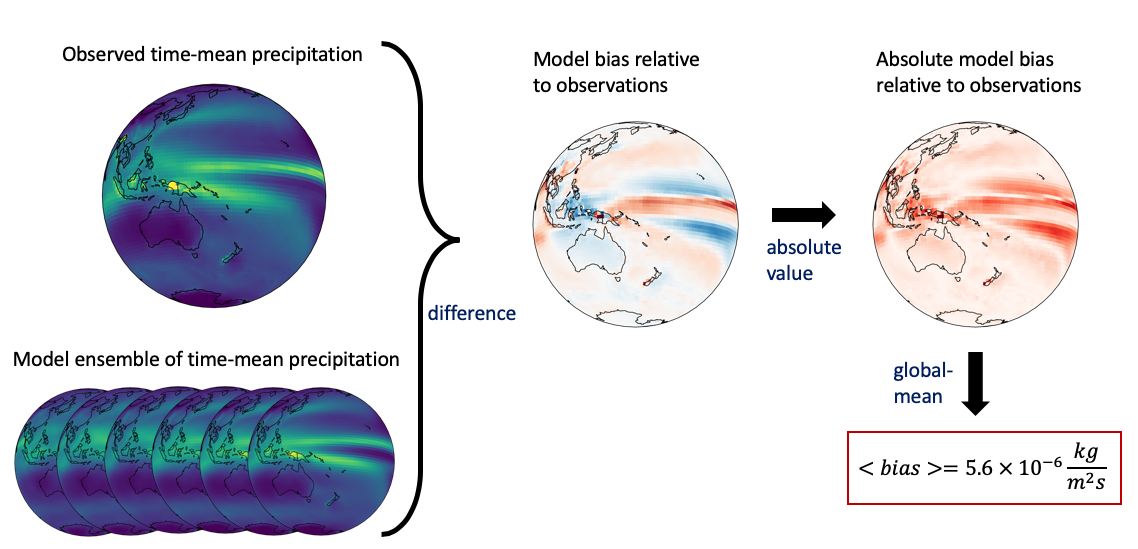
\includegraphics[width=1.0\textwidth]{figures/model_skill_schematic.png}
\centering
\caption{}
\label{fig.model_skill_flowchart}
\end{figure}

\section{Results}

\section{Discussion}

\section{Conclusion}

\bibliographystyle{apalike}
\bibliography{references.bib, refs_by_hand.bib}

\end{document}
